\documentclass[12pt,letterpaper]{article}
\usepackage[letterpaper,margin=1in]{geometry}
\usepackage[T1]{fontenc}
\usepackage{mathptmx}
\usepackage{microtype}
\usepackage[authoryear,round]{natbib}
\usepackage{xcolor}
\usepackage{tikz}
\usetikzlibrary{positioning,arrows.meta}
\usepackage[font=small,labelfont=bf,skip=5pt]{caption}
\usepackage{flafter}
\usepackage[colorlinks=true,citecolor=blue,linkcolor=black,urlcolor=black]{hyperref}
\usepackage{titlesec}
\setlength{\parindent}{0pt}
\setlength{\parskip}{5pt}
\setlength{\textfloatsep}{10pt plus 2pt minus 2pt}
\titleformat{\section}{\normalfont\normalsize\bfseries}{}{0pt}{}
\titlespacing*{\section}{0pt}{10pt}{3pt}
\newcommand{\rg}[1]{\par\vspace{3pt}{\normalfont\bfseries\itshape #1}\par\nopagebreak}
\newcommand{\task}[1]{\textbf{#1}\hspace{0.4em}}
\hypersetup{pdftitle={Trustworthy Collective Reasoning and Evaluation for AI Agents},pdfauthor={Xinya Du}}
\begin{document}
\begin{center}
{\large\bfseries Trustworthy Collective Reasoning and Evaluation for AI Agents\par}
\vspace{3pt}
Xinya Du, The University of Texas at Dallas (xinya.du@utdallas.edu)\par
ONR FY27 YIP white paper for Dr.\ Predrag Neskovic, Code 311, Mathematical Data Science\par
\end{center}

\section*{1\quad The problem}
Five AI agents read shipping reports and are asked whether a cargo vessel has left port. Three say yes and two say no, but the vessel is still in port. Two of the yes answers rest on the same outdated schedule, and the third comes from a compromised agent that argues confidently for yes. Nobody knows in advance which agents to trust. A majority vote picks the wrong answer, and open discussion may do no better, because the compromised agent is persuasive and the two agents with the same source back each other up.

\textbf{The central problem of this project is how a group of AI agents of unknown and correlated reliability, some possibly dishonest, can reach trustworthy decisions.}

The example shows three ways collective judgment fails. Agents that share a mistake are counted as independent votes. A dishonest agent can rate or argue strategically. And discussion rewards confidence and persistence, whether or not they come with evidence. Verifying every claim would prevent these failures, but trustworthy verification cannot rest on the agents' own judgment. Beyond simple automatic tests, it takes a person, such as an analyst or an expert, or a direct measurement, such as a replication or a satellite image, which are slow and costly. An AI verifier alone does not help, because it is one more agent of unknown reliability, and as AI agents produce more claims, the share that people can verify only shrinks.

\section*{2\quad Why it matters}
AI models now routinely grade one another's work, and multi-agent systems increasingly decide by vote or discussion \citep{zheng2023judging,verga2024juries}. Their agreement is weaker evidence than it looks, because their errors are correlated, and more so as models improve \citep{kim2025correlated,goel2025great}. In one study, nine AI judges carried the information of about two independent judges, and items on which all nine agreed were still wrong 9.1\% of the time \citep{kohli2026nine}. Discussion makes agreement even less informative: one round of debate raised a panel's unanimity from 39.5\% to 95.2\% with almost no change in accuracy \citep{shu2026unanimity}. Agents can also collude. When breaking a rule to verify each other's work paid more than following it, pairs of agents colluded in 94\% of runs across ten models \citep{shi2026collusion}.

Navy decisions face these problems together. AI tools differ in reliability that is rarely known in advance, the true answer often arrives late, an adversary may compromise an agent or plant false reports, and verification is costly or impossible when connectivity is limited. A commander must still decide whether to act on what the agents agree on.

\section*{3\quad How it is solved today, and the limitations}
Statistical methods estimate each rater's accuracy without an answer key \citep{dawid1979maximum,whitehill2009whose} and detect sources that copy one another \citep{dong2009dependence}, but they assume that raters err independently or in simple patterns \citep{jaffe2016dependent} and never change their minds. Two recent preprints estimate the accuracy and shared mistakes of AI judges from small trusted sets \citep{hossain2026agreement,zhu2026stopping}, treating the judges as honest and as never conferring.

Computational social choice designs mechanisms in which a participant's ratings of others cannot change its own chance of selection, as in impartial peer review \citep{kurokawa2015impartial,alon2011sum}, along with fair panel selection \citep{flanigan2021fair}. \citet{lev2023peernomination} added reliability weights to impartial selection, but their weights reward agreeing with the majority, and the authors note that accurate reviewers can no longer be identified once they are half or fewer. These mechanisms take opinions as given. In our setting there is a correct answer, some claims can be verified, and opinions change as agents talk.

Letting models debate can help \citep{du2024debate}, but majority voting explains most of the gain \citep{choi2025debate}, and a single persuasive adversary can cut a group's accuracy by 10\% to 40\% \citep{amayuelas2024attack}. A recent collaborative version of AI safety debate \citep{irving2018debate,khan2024debating} raised weak-judge accuracy to 62.1\%, from 49.2\% with standard debate, but its judges accepted the models' consensus almost every time, even when both were wrong, and it assumes honest models \citep{jiang2026disagreement}. No existing approach learns whom to trust from verified outcomes while resisting dishonest or colluding agents.

\section*{4\quad Our approach: what is new, and why it will succeed}
Our approach rests on one idea: use verified results, including a few audits that agents cannot predict, to decide whom to trust, to settle disputes, and to reward good behavior. Each agent first answers on its own, as a list of claims, each citing the source it rests on. Automatic tests, run by software, cover every claim: does a quotation match its source, or does an online record agree? Audits are done by a person, such as an analyst or an expert, or by a direct measurement, such as a satellite image; they are costly, so only a few claims get one, some chosen at random. As with random tax audits, no agent knows which claims will be audited, so dishonesty is risky. Figure~\ref{fig:overview} shows how the three research goals (RGs) use tests and audits.

\begin{figure}[!t]
\centering
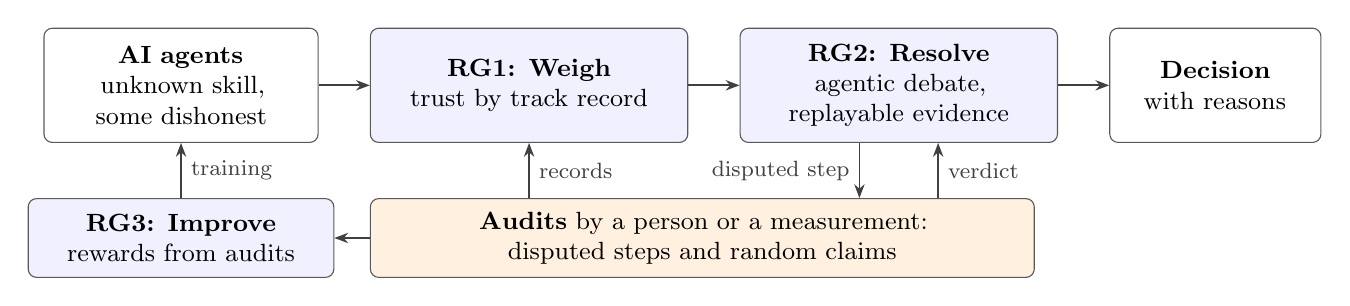
\begin{tikzpicture}[font=\small,
  box/.style={draw=black!65, rounded corners=3pt, align=center, inner sep=4pt, execute at begin node={\hyphenpenalty=10000}},
  top/.style={box, minimum height=1.45cm},
  bot/.style={box, minimum height=1.0cm},
  arr/.style={-{Stealth[length=5pt]}, semithick, black!75},
  lab/.style={font=\footnotesize, text=black!75}]
\node[top, text width=3.2cm] (ag) {\textbf{AI agents}\\unknown skill, some dishonest};
\node[top, text width=3.75cm, fill=blue!6, right=0.65cm of ag] (r1) {\textbf{RG1: Weigh}\\trust by track record};
\node[top, text width=3.75cm, fill=blue!6, right=0.65cm of r1] (r2) {\textbf{RG2: Resolve}\\agentic debate, replayable evidence};
\node[top, text width=2.4cm, right=0.65cm of r2] (dec) {\textbf{Decision}\\with reasons};
\node[bot, text width=8.15cm, fill=orange!12, anchor=north west] (ck) at ([yshift=-0.7cm]r1.south west) {\textbf{Audits} by a person or a measurement: disputed steps and random claims};
\node[bot, text width=3.6cm, fill=blue!6, anchor=north] (r3) at ([yshift=-0.7cm]ag.south) {\textbf{RG3: Improve}\\rewards from audits};
\draw[arr] (ag) -- (r1);
\draw[arr] (r1) -- (r2);
\draw[arr] (r2) -- (dec);
\draw[arr] (r1.south |- ck.north) -- node[lab, right]{records} (r1.south);
\draw[arr] ([xshift=-5mm]r2.south) -- node[lab, left]{disputed step} ([xshift=-5mm]r2.south |- ck.north);
\draw[arr] ([xshift=5mm]r2.south |- ck.north) -- node[lab, right]{verdict} ([xshift=5mm]r2.south);
\draw[arr] (ck.west) -- (ck.west -| r3.east);
\draw[arr] (r3) -- node[lab, right]{training} (ag);
\end{tikzpicture}
\caption{Overview. RG1 weighs agents by their track record; RG2 settles disputes by agentic debate with replayable evidence, plus audits; RG3 rewards messages that tests and audits confirm.}
\label{fig:overview}
\end{figure}

\rg{RG1. Weigh agents by their track record}
Agents differ in skill, often by topic, and agents built on similar models make the same mistakes.

\task{Task 1.1: Weights that count shared mistakes once.} We will estimate each agent's accuracy, and which agents tend to be wrong together, from the results of tests and audits. The core method extends the classic rater model of \citet{dawid1979maximum} with shared error factors: agents that keep failing the same tests and audits share a factor, and agreement within a factor adds little evidence. In the vessel example, the two agents that used the same outdated schedule would count about once. Our PRD method weighted each AI judge by how its peers rated its answers \citep{li2024prd}; here the weights come from tests and audits instead.

\task{Task 1.2: Impartial peer ratings.} When agents also rate one another, as on our PeerEval leaderboard (peereval-ai.github.io), an agent could raise its own standing by downgrading rivals; in PRD, a lower score for a rival also lowered that rival's weight as a judge. We adapt impartial peer review \citep{kurokawa2015impartial} using the partition idea of \citet{alon2011sum}: agents are split into groups, with agents built on the same base model in the same group, and each group fills a fixed number of top places with the members rated highest by agents outside it. An agent's ratings therefore never change its own outcome. \citet{lev2023peernomination} weight raters by agreement with the majority; we weight them by their track records from Task 1.1.

\rg{RG2. Settle disputes and catch wrong agreement}
Text-only debate rewards persuasion, and agreement can hide shared mistakes or collusion.

\task{Task 2.1: Agentic debate with replayable evidence.} When weighted agents still disagree, they debate as agents with tools, such as search, code execution, and database queries, in a shared sandbox, building on PRD's peer discussion and HiPRAG's search agents. Agents with the same answer send one representative, the one with the best track record, so a majority gets no extra voice; majority pressure is known to suppress correction in debate \citep{wu2025really}. Following prover--estimator debate \citep{browncohen2025prover}, one side splits its argument into steps, the other states how likely each step is, and the debate recurses into the step whose estimate the first side disputes, so a flaw cannot hide in a long chain. Every step must carry the tool calls behind its evidence, and the judge, itself an agent with the same tools \citep{zhuge2025agent}, replays them; evidence that does not replay carries no weight. Unlike tool-using debates in which the judge still weighs arguments \citep{jeong2026toolmad}, replay turns each disputed step into a new automatic test; only steps that replay cannot settle are audited. In the vessel example, a replayed query shows the schedule was superseded, and one satellite image settles the rest.

\task{Task 2.2: Planted cases against collusion.} Debate starts only when agents disagree, but agents that share a mistake or collude simply agree. We therefore mix in planted cases whose answer we know, such as a paper with a deliberately inserted error, as in studies of human peer review \citep{schroter2008errors}. Agents that fail the same planted cases are flagged as a group, and planted collusion examples test whether a judge model reading the agents' messages catches them, like the honeypots of AI control \citep{greenblatt2024control}. Because capable models can often spot planted cases \citep{needham2025evaluated}, random audits of real claims confirm that agents behave alike on both.

\rg{RG3. Train agents that contribute evidence}
Rewarding persuasion has produced agents that fabricate quotations \citep{kenton2026debate} and mislead people \citep{wen2025mislead}.

\task{Task 3: Rewards for verified contributions.} We will train agents with reinforcement learning, rewarding each message by its verified effect: an agent earns reward when its message moves the group toward an answer that a test or audit confirms, and loses reward when that answer is refuted. This extends the PI's process reward models, FG-PRM and HiPRAG \citep{li2025fgprm,wu2026hiprag}, from the steps of one agent to the messages of many. The main experiment compares training to contribute with training to win debates \citep{arnesen2024selfplay}.

\rg{Evaluation: testbeds and a red-team test}
All data are synthetic or public. We will use (A) math and code problems solved by agents of known skill, some given the same flawed hint; (B) questions over many documents, built with our MEQA pipeline \citep{li2024meqa} and including synthetic maritime scenarios; and (C) scientific claims and peer review, with reproducibility studies as audits. In the testbeds, an audit reveals the stored correct answer, and each method gets a fixed audit budget. Following the AI control methodology \citep{greenblatt2024control}, a red team will train agents to collude, to spot planted cases, and to cheat only when they expect no audit, and we will measure how many wrong decisions get through as the audit budget varies. Baselines are majority vote, standard rater weighting, our PRD, text-only and tool-using debate \citep{jiang2026disagreement,jeong2026toolmad}, and recent judge-weighting methods \citep{hossain2026agreement,zhu2026stopping,lev2023peernomination}.

\textbf{What is new.} (i) Trust is learned from audits and planted cases that agents cannot predict, and agents that share mistakes count once. (ii) Debaters and judge are tool-using agents, the judge replays each step's evidence, and only what replay cannot settle is audited. (iii) Agents are rewarded for evidence that tests and audits confirm, instead of for winning arguments.

\textbf{Why it will succeed.} Theory backs the central idea. Without trusted audits, dishonest raters who imitate honest ones cannot be told apart from them, while a number of audits that does not grow with the number of items suffices even when honest raters are a minority \citep{steinhardt2016avoiding}; occasional audits also motivate honest effort better than many schemes that only compare agents with one another \citep{gao2019incentivizing}. Each task builds on the PI's own tools; for example, PRD agrees better with human judgments than the strongest single AI judge \citep{li2024prd}, and HiPRAG cuts unnecessary searches to 2.3\% \citep{wu2026hiprag}. The PI co-led one of five red teams in the Amazon Nova AI Challenge, holds a 2024 NSF CAREER award and a 2023 Amazon Research Award, and as a postdoctoral researcher led system integration for RESIN-11 in DARPA KAIROS.

\section*{5\quad Limitations of our approach}
If a disputed step can be neither tested nor audited, or if every agent shares the same misconception, no method can recover the truth; ours then reports the claim as unresolved. Audits can themselves be wrong, so we will measure how sensitive the methods are to faulty audits. A group that cheats only once, on a single high-stakes claim, may succeed before it is caught; we can bound such losses but not rule them out. Agents may also coordinate through hidden signals that monitoring does not catch \citep{mathew2025hidden}, so robustness is shown only for the behaviors we test. Operational Navy use would require Navy data and expert validation.

\section*{6\quad Impact if successful}
The project will show when agreement among AI agents counts as evidence, and how few audits it takes to make it count. A Navy analyst using several AI tools would get a decision together with its reasons: which tools' judgments carried weight and why, which claim is still disputed, and when a person should look. Each goal meets a Navy need: tools of unknown reliability (RG1), scarce audits (RG2), and agents that report evidence (RG3). The same methods would let conferences and funding agencies test impartial, audited peer review with AI reviewers. We will release code, testbeds, and protocols.

\clearpage
\begingroup
\small
\setlength{\bibsep}{3pt}
\begin{thebibliography}{}
\setlength{\itemsep}{2.5pt}
\bibitem[{Alon et~al.(2011)}]{alon2011sum} N. Alon, F. Fischer, A. D. Procaccia, and M. Tennenholtz (2011). \href{https://doi.org/10.1145/2000378.2000390}{Sum of Us: Strategyproof Selection from the Selectors}. TARK, pp. 101--110.
\bibitem[{Amayuelas et~al.(2024)}]{amayuelas2024attack} A. Amayuelas, X. Yang, A. Antoniades, W. Hua, L. Pan, and W. Y. Wang (2024). \href{https://arxiv.org/abs/2406.14711}{MultiAgent Collaboration Attack: Investigating Adversarial Attacks in Large Language Model Collaborations via Debate}. Findings of EMNLP, pp. 6929--6948.
\bibitem[{Arnesen et~al.(2024)}]{arnesen2024selfplay} S. Arnesen, D. Rein, and J. Michael (2024). \href{https://arxiv.org/abs/2409.16636}{Training Language Models to Win Debates with Self-Play Improves Judge Accuracy}. arXiv:2409.16636.
\bibitem[{Brown-Cohen et~al.(2025)}]{browncohen2025prover} J. Brown-Cohen, G. Irving, G. Piliouras, L. Chen, J. Li, and Z. Xun (2025). \href{https://arxiv.org/abs/2506.13609}{Avoiding Obfuscation with Prover-Estimator Debate}. arXiv:2506.13609.
\bibitem[{Choi et~al.(2025)}]{choi2025debate} H. K. Choi, X. Zhu, and S. Li (2025). \href{https://arxiv.org/abs/2508.17536}{Debate or Vote: Which Yields Better Decisions in Multi-Agent Large Language Models?} NeurIPS.
\bibitem[{Dawid and Skene(1979)}]{dawid1979maximum} A. P. Dawid and A. M. Skene (1979). \href{https://doi.org/10.2307/2346806}{Maximum Likelihood Estimation of Observer Error-Rates Using the EM Algorithm}. Journal of the Royal Statistical Society, Series C (Applied Statistics) 28(1):20--28.
\bibitem[{Dong et~al.(2009)}]{dong2009dependence} X. L. Dong, L. Berti-Equille, and D. Srivastava (2009). \href{https://doi.org/10.14778/1687627.1687689}{Integrating Conflicting Data: The Role of Source Dependence}. PVLDB 2(1):550--561.
\bibitem[{Du et~al.(2024)}]{du2024debate} Y. Du, S. Li, A. Torralba, J. B. Tenenbaum, and I. Mordatch (2024). \href{https://proceedings.mlr.press/v235/du24e.html}{Improving Factuality and Reasoning in Language Models through Multiagent Debate}. ICML, PMLR 235:11733--11763.
\bibitem[{Flanigan et~al.(2021)}]{flanigan2021fair} B. Flanigan, P. G\"olz, A. Gupta, B. Hennig, and A. D. Procaccia (2021). \href{https://doi.org/10.1038/s41586-021-03788-6}{Fair Algorithms for Selecting Citizens' Assemblies}. Nature 596:548--552.
\bibitem[{Gao et~al.(2019)}]{gao2019incentivizing} A. Gao, J. R. Wright, and K. Leyton-Brown (2019). \href{https://doi.org/10.1016/j.artint.2019.03.004}{Incentivizing Evaluation with Peer Prediction and Limited Access to Ground Truth}. Artificial Intelligence.
\bibitem[{Goel et~al.(2025)}]{goel2025great} S. Goel, J. Str\"uber, I. A. Auzina, K. K. Chandra, P. Kumaraguru, D. Kiela, A. Prabhu, M. Bethge, and J. Geiping (2025). \href{https://proceedings.mlr.press/v267/goel25b.html}{Great Models Think Alike and this Undermines AI Oversight}. ICML, PMLR 267:19621--19678.
\bibitem[{Greenblatt et~al.(2024)}]{greenblatt2024control} R. Greenblatt, B. Shlegeris, K. Sachan, and F. Roger (2024). \href{https://arxiv.org/abs/2312.06942}{AI Control: Improving Safety Despite Intentional Subversion}. ICML, PMLR 235:16295--16336.
\bibitem[{Hossain et~al.(2026)}]{hossain2026agreement} E. Hossain, N. Yousefi, and S.-N. Lim (2026). \href{https://arxiv.org/abs/2609.22512}{Agreement Overstates Evidence: Error Dependence in LLM Judge Consensus}. arXiv:2609.22512.
\bibitem[{Irving et~al.(2018)}]{irving2018debate} G. Irving, P. Christiano, and D. Amodei (2018). \href{https://arxiv.org/abs/1805.00899}{AI Safety via Debate}. arXiv:1805.00899.
\bibitem[{Jaffe et~al.(2016)}]{jaffe2016dependent} A. Jaffe, E. Fetaya, B. Nadler, T. Jiang, and Y. Kluger (2016). \href{https://proceedings.mlr.press/v51/jaffe16.html}{Unsupervised Ensemble Learning with Dependent Classifiers}. AISTATS, PMLR 51:351--360.
\bibitem[{Jeong et~al.(2026)}]{jeong2026toolmad} S. Jeong, Y. Choi, J. Kim, and B. Jang (2026). \href{https://arxiv.org/abs/2601.04742}{Tool-MAD: A Multi-Agent Debate Framework for Fact Verification with Diverse Tool Augmentation and Adaptive Retrieval}. arXiv:2601.04742.
\bibitem[{Jiang et~al.(2026)}]{jiang2026disagreement} Y. Jiang, C. Chen, T. Wu, L. Sun, H. Liu, S. Feng, and C. Tan (2026). \href{https://arxiv.org/abs/2607.01251}{Collaborative Disagreement Resolution for Scalable Oversight}. ICML.
\bibitem[{Kenton et~al.(2026)}]{kenton2026debate} Z. Kenton, L. Janzer, R. Greig, T. H. Teh, K. Tyshchuk, J. Brown-Cohen, H. Edwards, S. Rajamanoharan, N. Y. Siegel, N. Jaques, and R. Shah (2026). \href{https://arxiv.org/abs/2608.17776}{Debate Training Reduces Reward Hacking in RLAIF}. arXiv:2608.17776.
\bibitem[{Khan et~al.(2024)}]{khan2024debating} A. Khan et al. (2024). \href{https://proceedings.mlr.press/v235/khan24a.html}{Debating with More Persuasive LLMs Leads to More Truthful Answers}. ICML, PMLR 235:23662--23733.
\bibitem[{Kim et~al.(2025)}]{kim2025correlated} E. M. Kim, A. Garg, K. Peng, and N. Garg (2025). \href{https://proceedings.mlr.press/v267/kim25e.html}{Correlated Errors in Large Language Models}. ICML, PMLR 267:30038--30066.
\bibitem[{Kohli(2026)}]{kohli2026nine} G. Kohli (2026). \href{https://arxiv.org/abs/2605.29800}{Nine Judges, Two Effective Votes: Correlated Errors Undermine LLM Evaluation Panels}. arXiv:2605.29800.
\bibitem[{Kurokawa et~al.(2015)}]{kurokawa2015impartial} D. Kurokawa, O. Lev, J. Morgenstern, and A. D. Procaccia (2015). \href{https://www.ijcai.org/Abstract/15/088}{Impartial Peer Review}. IJCAI, pp. 582--588.
\bibitem[{Lev et~al.(2023)}]{lev2023peernomination} O. Lev, N. Mattei, P. Turrini, and S. Zhydkov (2023). \href{https://doi.org/10.1016/j.artint.2022.103843}{PeerNomination: A Novel Peer Selection Algorithm to Handle Strategic and Noisy Assessments}. Artificial Intelligence 316:103843.
\bibitem[{Li et~al.(2024a)}]{li2024prd} R. Li, T. Patel, and X. Du (2024a). \href{https://openreview.net/forum?id=YVD1QqWRaj}{PRD: Peer Rank and Discussion Improve Large Language Model based Evaluations}. TMLR.
\bibitem[{Li et~al.(2024b)}]{li2024meqa} R. Li, Z. Wang, S. Q. Tran, L. Xia, and X. Du (2024b). \href{https://proceedings.neurips.cc/paper_files/paper/2024/hash/e560a0b22e4432003d0dba63ff8dc457-Abstract.html}{MEQA: A Benchmark for Multi-hop Event-centric Question Answering with Explanations}. NeurIPS 37, Datasets and Benchmarks, pp. 126835--126862.
\bibitem[{Li et~al.(2025)}]{li2025fgprm} R. Li, Z. Luo, and X. Du (2025). \href{https://aclanthology.org/2025.findings-emnlp.228/}{FG-PRM: Fine-grained Hallucination Detection and Mitigation in Language Model Mathematical Reasoning}. Findings of EMNLP, pp. 4247--4278.
\bibitem[{Mathew et~al.(2025)}]{mathew2025hidden} Y. Mathew, O. Matthews, R. McCarthy, J. Velja, C. Schroeder de Witt, D. Cope, and N. Schoots (2025). \href{https://aclanthology.org/2025.ijcnlp-long.34/}{Hidden in Plain Text: Emergence and Mitigation of Steganographic Collusion in LLMs}. IJCNLP-AACL, pp. 585--624.
\bibitem[{Needham et~al.(2025)}]{needham2025evaluated} J. Needham, G. Edkins, G. Pimpale, H. Bartsch, and M. Hobbhahn (2025). \href{https://arxiv.org/abs/2505.23836}{Large Language Models Often Know When They Are Being Evaluated}. arXiv:2505.23836.
\bibitem[{Schroter et~al.(2008)}]{schroter2008errors} S. Schroter, N. Black, S. Evans, F. Godlee, L. Osorio, and R. Smith (2008). \href{https://doi.org/10.1258/jrsm.2008.080062}{What Errors Do Peer Reviewers Detect, and Does Training Improve Their Ability to Detect Them?} Journal of the Royal Society of Medicine 101(10):507--514.
\bibitem[{Shi et~al.(2026)}]{shi2026collusion} X. Shi, Y. Zhang, and D. Yang (2026). \href{https://arxiv.org/abs/2609.24967}{Emergent Collusion in Long-Horizon LLM Agent Interaction}. arXiv:2609.24967.
\bibitem[{Shu(2026)}]{shu2026unanimity} Y. Shu (2026). \href{https://arxiv.org/abs/2609.26145}{Unanimity Without Persuasion: A Single Round of Debate Erases the Disagreement That Verification Needs}. arXiv:2609.26145.
\bibitem[{Steinhardt et~al.(2016)}]{steinhardt2016avoiding} J. Steinhardt, G. Valiant, and M. Charikar (2016). \href{https://arxiv.org/abs/1606.05374}{Avoiding Imposters and Delinquents: Adversarial Crowdsourcing and Peer Prediction}. NeurIPS 29.
\bibitem[{Verga et~al.(2024)}]{verga2024juries} P. Verga et al. (2024). \href{https://arxiv.org/abs/2404.18796}{Replacing Judges with Juries: Evaluating LLM Generations with a Panel of Diverse Models}. arXiv:2404.18796.
\bibitem[{Wen et~al.(2025)}]{wen2025mislead} J. Wen, R. Zhong, A. Khan, E. Perez, J. Steinhardt, M. Huang, S. R. Bowman, H. He, and S. Feng (2025). \href{https://arxiv.org/abs/2409.12822}{Language Models Learn to Mislead Humans via RLHF}. ICLR.
\bibitem[{Whitehill et~al.(2009)}]{whitehill2009whose} J. Whitehill, P. Ruvolo, T. Wu, J. Bergsma, and J. Movellan (2009). \href{https://proceedings.neurips.cc/paper/2009/hash/f899139df5e1059396431415e770c6dd-Abstract.html}{Whose Vote Should Count More: Optimal Integration of Labels from Labelers of Unknown Expertise}. NeurIPS 22, pp. 2035--2043.
\bibitem[{Wu et~al.(2025)}]{wu2025really} H. Wu, Z. Li, and L. Li (2025). \href{https://arxiv.org/abs/2511.07784}{Can LLM Agents Really Debate? A Controlled Study of Multi-Agent Debate in Logical Reasoning}. arXiv:2511.07784.
\bibitem[{Wu et~al.(2026)}]{wu2026hiprag} P. Wu, M. Zhang, K. Wan, W. Zhao, K. He, X. Du, and Z. Chen (2026). \href{https://proceedings.iclr.cc/paper_files/paper/2026/hash/85255cf8f2d2318cc7cffd0b1bc66625-Abstract-Conference.html}{HiPRAG: Hierarchical Process Rewards for Efficient Agentic Retrieval Augmented Generation}. ICLR.
\bibitem[{Zheng et~al.(2023)}]{zheng2023judging} L. Zheng et al. (2023). \href{https://proceedings.neurips.cc/paper_files/paper/2023/hash/91f18a1287b398d378ef22505bf41832-Abstract.html}{Judging LLM-as-a-Judge with MT-Bench and Chatbot Arena}. NeurIPS 36, Datasets and Benchmarks, pp. 46595--46623.
\bibitem[{Zhu et~al.(2026)}]{zhu2026stopping} B. Zhu, Y. Xie, and Y. Rao (2026). \href{https://arxiv.org/abs/2608.19802}{Stopping and Routing LLM Judge Panels}. arXiv:2608.19802.
\bibitem[{Zhuge et~al.(2025)}]{zhuge2025agent} M. Zhuge, C. Zhao, D. Ashley, W. Wang, D. Khizbullin, Y. Xiong, Z. Liu, E. Chang, R. Krishnamoorthi, Y. Tian, Y. Shi, V. Chandra, and J. Schmidhuber (2025). \href{https://arxiv.org/abs/2410.10934}{Agent-as-a-Judge: Evaluate Agents with Agents}. ICML.
\end{thebibliography}
\endgroup
\end{document}
